% ---------------------------------------------------------------------
% ---------------------------------------------------------------------
% ---------------------------------------------------------------------

\chapter[Introduction, contents and aims of the thesis]{Introduction, contents and aims of the thesis}



% ---------------------------------------------------------------------
% ---------------------------------------------------------------------
\section{Introduction}
\label{sec:Intro}

\section{Characteristics of omic data}
\label{sec:charomicdata}
Data sets have experienced a rapid growth in size and complexity during the last years, and biology and biomedicine have been no exception \parencite{marx2013biology}. Few decades ago, a typical data set consisted in dozens of variables, and a large data set was one with some few hundreds of variables. Nowadays, the different omic technologies have evolved producing data sets ranging from hundreds of variables, in the case of specific panels or targeted analyses, to thousands or even hundreds of thousands of variables for untargeted or whole genome analyses. A specific characteristic of omic data sets, compared to data sets from other disciplines is their heterogeneous nature. Individual variability is huge and experiments have to be repeated many times to reach conclusions. This has lead to the so called "reproducibility crisis", which considers that many research findings could be false \parencite{ioannidis2005most, begley2015reproducibility}. In fact, some studies have estimated that more than 70\% of published works in the field of biology may be not reproducible \parencite{baker20161}.
Omic data can be classified according to the nature of the elements being analyzed. Following this approach, 5 different fields can be delimited (\autoref{figura01}):
\begin{itemize}
    \item Genomics: Focused at the genes level (DNA)
    \item Epigenomics: Studies the reversible modifications of the genome, which regulate expression
    \item Transcriptomics: Focused at the RNA level
    \item Proteomics: Focused at the protein level
    \item Metabolomics: Studies metabolites in a biological entity, which are the end products of cellular processes
\end{itemize}

\begin{figure}[htbp]\centering
		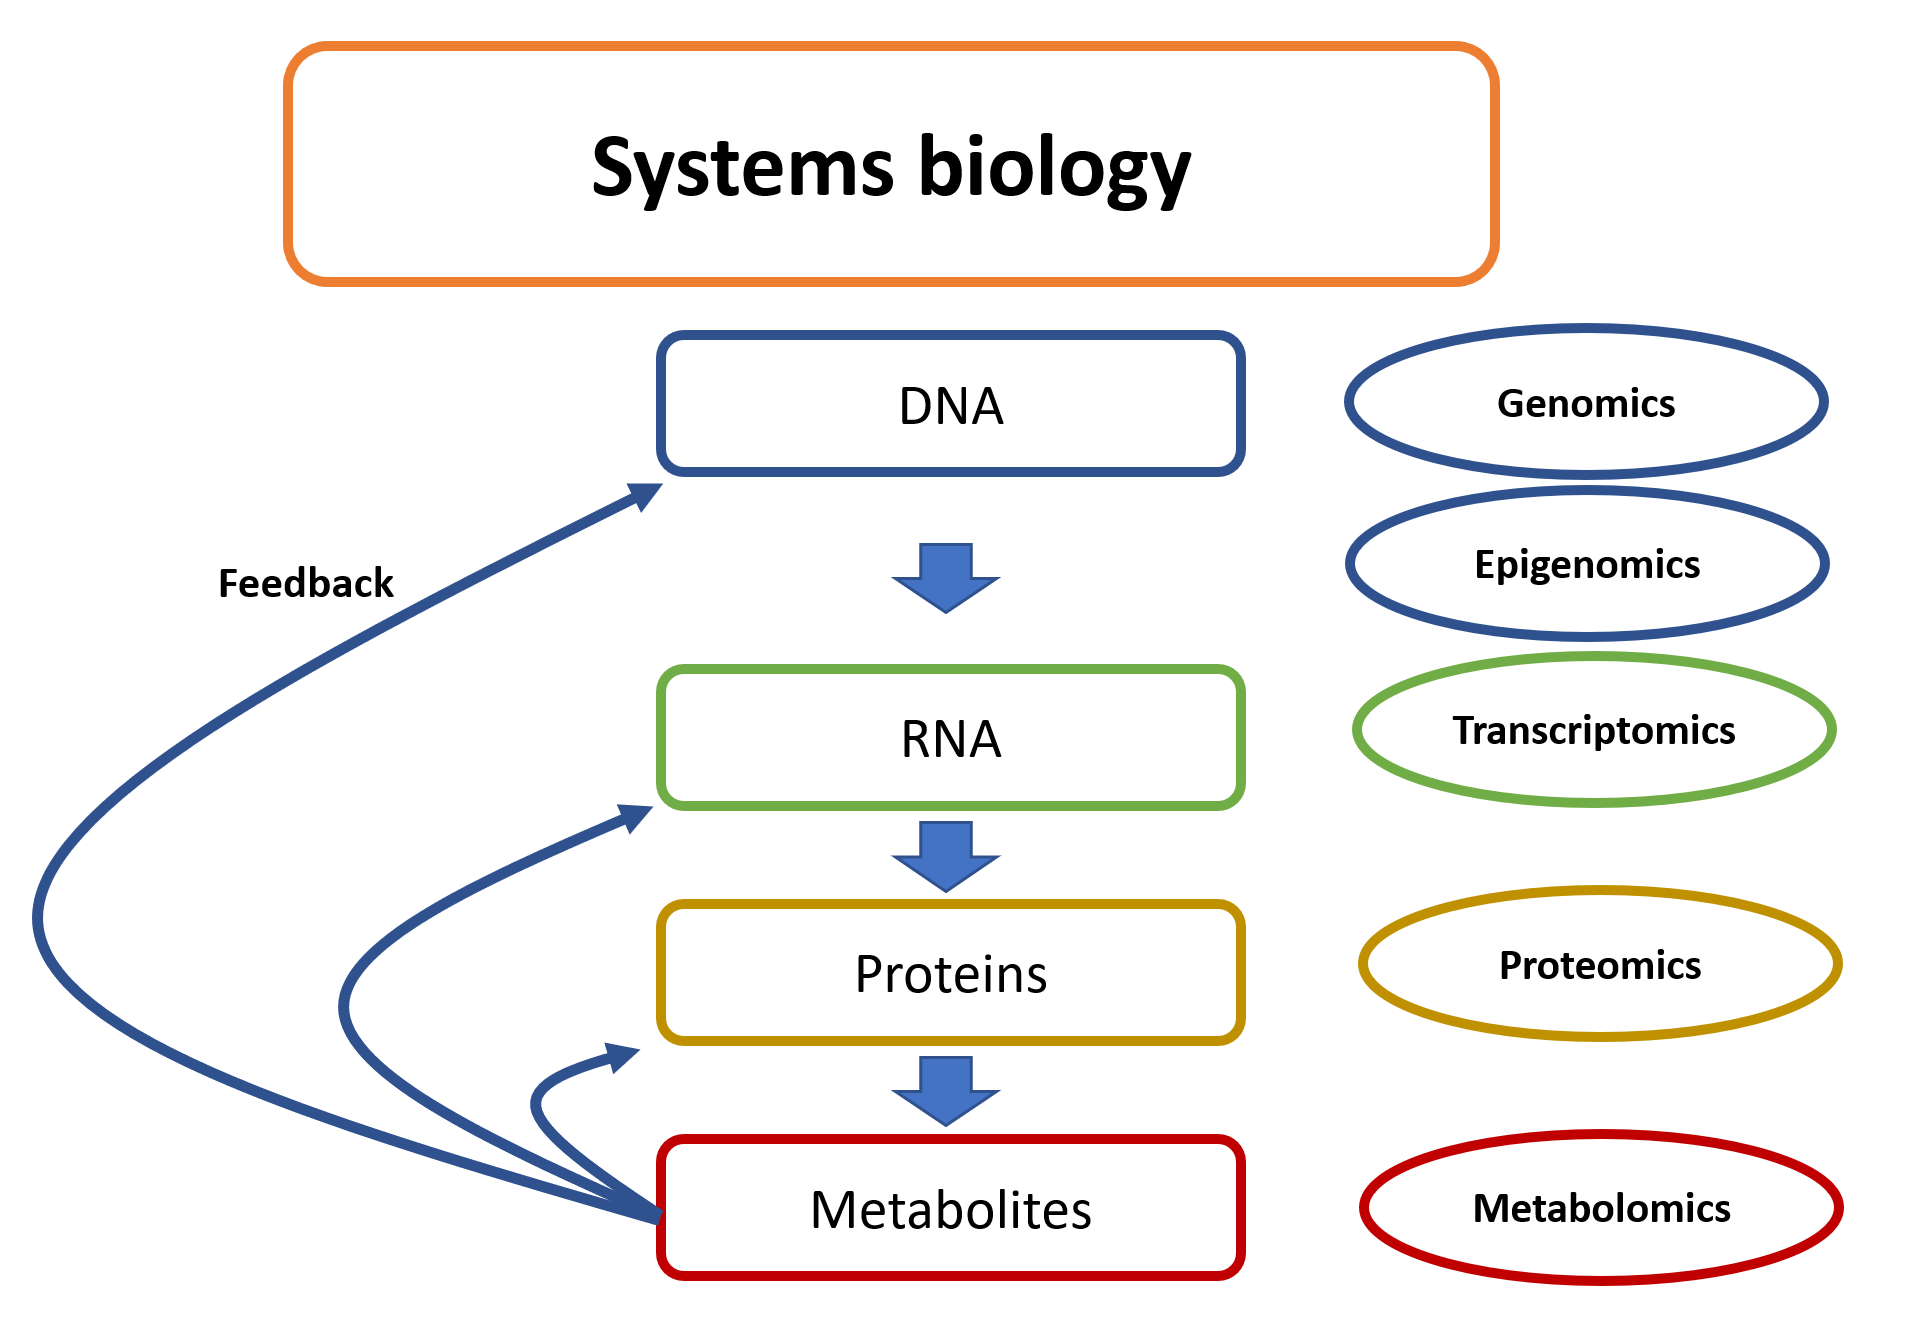
\includegraphics[width=.7\textwidth]{figura01}
		\caption{Different omic technologies and their relationship}
		\label{figura01}
	\end{figure}

\subsection{Metabolomic data}
The term '\textit{metabolome}' is used to address the entire set of metabolites present in an organism and '\textit{metabolomics}' is defined as the comprehensive and quantitative analysis of all metabolites of the biological system under study \parencite{fiehn2001combining}. In general metabolomic studies can be classified as targeted or untargeted depending on whether the researcher measures and quantifies a specific set of known metabolites or the largest possible number of metabolites contained in a biological system. 
Among all omic technologies, metabolomics is the most complex and heterogeneous. In genomics, epigenomics and transcriptomics, measurement procedures are reasonably standardized. This is not the case in metabolomics, with many different technologies being used, which lead to different study designs and different produced data types \parencite{moco2007metabolomics}. The commonly used analytical techniques for metabolomic studies are nuclear magnetic resonance (NMR), spectroscopy and mass spectrometry \parencite{buscher2009cross}. Another specific hurdle of metabolomics is the identification of the metabolites in untargeted analyses. Many of the metabolites found in an untargeted analysis can not be identified, because the data bases for associating a specific mass and retention time to a concrete metabolite are still very immature \parencite{mathew2013metabolomics}. In fact, identification of unknowns is considered as the bottleneck of untargeted metabolomics \parencite{bingol2018recent}.
In any case, although heterogeneous, metabolomic data share a common set of properties which define their most important characteristics for their statistical analysis:

\begin{itemize}
    \item High correlation among variables
    \item Complex pre-processing of the signal to obtain the data
    \item High range of detection values among variables
    \item Variables (metabolites) found in one analysis are not guaranteed to be found in a subsequent analysis
\end{itemize}

All these properties add to the difficulty of analyzing metabolomic data, as will be further developed in the next section.

\section{Challenges for analyzing metabolomic data}
\label{sec:challengesmetabodata}
Traditionally, omic data analyses have been performed using classical statistical methods from last century. In most cases, these methods consisted in bivariate tests such as \textit{t test} or \textit{Wilcoxon-Mann Whitney test}, followed by some sort of multiple comparissons correction such as \textit{Bonferroni} or \textit{False Discovery Rate} \parencite{hochberg1990more, benjamini1995controlling}. These approaches suffer from several drawbacks including lack of statistical power, lack of interpretability of results, and omission of complex relationships among variables. Thus, classical statistical methods based on bivariate tests are not adequate to extract all the information available in omic data sets.
Some of the mentioned problems such as the lack of interpretability or the omission of complex relationships could be adressed using statistical models such as linear models or generalized liner models, but these methods also suffer from other problems when dealing with omic data, such as the large number of variables and low sample size, which produces overfitting, and the high correlation among variables, which produces multicollinearity. All these obstacles for omic data analysis have motivated the development of numerous novel statistical techniques during the last decades specifically aimed at solving them. Methods such as PLS \parencite{wold1984collinearity}, lasso \parencite{tibshirani1996regression}, elastic net \parencite{zou2005regularization} and random forest \parencite{breiman2001random}, among others, can deal with most of the problems exposed in the preceding lines. Nevertheless, other challenges remain partially unresolved, such as the analysis of repeated measures data or, more generally, data organized in multiway arrays. Also, in a discipline where the number of variables is so large, the development of variable selection methods is of utmost importance.

\section{Strategies and aims of the thesis}
\label{sec:strategiesthesis}


